\documentclass[12pt]{book}
%\reversemarginpar
%\usepackage[pass]{geometry} %important
%\newgeometry{a4paper,top=2.5cm,left=1.2in,right=1.2in,headheight=1.7cm,headsep=.3cm,marginpar=2cm,
%marginparsep=10pt,textheight=49\baselineskip}

\usepackage{lipsum,pgf,caption}
\usepackage{tikz}
\usetikzlibrary{decorations,decorations.shapes,shapes,fadings,patterns}
     % We need lots of libraries...
        \usetikzlibrary{
          arrows,
          calc,
          fit,
          patterns,
          plotmarks,
          shapes.geometric,
          shapes.misc,
          shapes.symbols,
          shapes.arrows,
          shapes.callouts,
          shapes.multipart,
%          shapes.gates.logic.US,
%          shapes.gates.logic.IEC,
%          circuits.logic.US,
%          circuits.logic.IEC,
%          circuits.logic.CDH,
%          circuits.ee.IEC,
%          datavisualization,
          datavisualization.formats.functions,
          er,
          automata,
          backgrounds,
          chains,
          topaths,
          trees,
          petri,
          mindmap,
          matrix,
          calendar,
          folding,
          fadings,
          shadings,
          spy,
          through,
          turtle,
          positioning,
          scopes,
          decorations.fractals,
          decorations.shapes,
          decorations.text,
          decorations.pathmorphing,
          decorations.pathreplacing,
          decorations.footprints,
          decorations.markings,
          shadows,
%          lindenmayersystems,
          intersections,
          fixedpointarithmetic,
          fpu,
          svg.path,
%          external,
        }


\IfFileExists{changepage.sty}{%
  \PassOptionsToPackage{strict}{changepage}
  \RequirePackage{changepage}
  }{}
\usepackage[strict]{changepage}
\def\aspectratio{\pgfmathparse{\paperheight/\paperwidth} \pgfmathresult}
\newpage
\newlength\innermargin

\def\printgeometryvalues{\leavevmode
paperwidth \the\paperwidth\\
paperheight \the\paperheight\\
theheadheight \the\headheight\\
theheadsep \the\headsep\\
thetopmargin \the\topmargin\\
theoddsidemargin \the\oddsidemargin\\
theevensidemargin\the\evensidemargin\\
thetextheight\the\textheight\\
thetextwidth \the\textwidth\\
themarginparsep \the\marginparsep\\
themarginparwidth \the\marginparwidth\\
themarginpush \the\marginparpush\\
thevoffset \the\voffset\\
thefootskip \the\footskip\\
aspect ratio \aspectratio\\
topskip \the\topskip\\
voffset \the\voffset\\
hoffset \the\hoffset\\
topmargin\the\topmargin}

\def\alignedge{%
  \checkoddpage%
  \parindent0pt%
%   \ifoddpage \global\setlength\innermargin{\oddsidemargin}
%          \else \global\setlength\innermargin{\evensidemargin}
%      \fi%
%   \if@twoside\setlength\innermargin{\dimexpr(\evensidemargin-\marginparsep)}%
%             \else\let\innermargin\oddsidemargin\fi
\ifoddpage \innermargin\oddsidemargin\else\innermargin\evensidemargin\fi
 }

\parindent0pt

%\pagecolor{brown}
%\color{white}
%\setlength\topmargin{10pt}
\makeatletter
% Set to true to draw an oddside page. Initially set to false.
\newcommand\layoutscale@cx{0.5}
\newif\ifoddpagelayout@cx
   \oddpagelayout@cxfalse
% Set true to draw marginpars on a page
\newif\ifdrawmarginpars
   \drawmarginparsfalse
\begin{document}
\mainmatter
\pagestyle{plain}
\null\newpage
\checkoddpage
\alignedge
\pgfmathsetmacro\tol{3mm}
\def\printlayout{%
\begin{tikzpicture}[scale=\layoutscale@cx,font={\footnotesize\sffamily},line width=.6pt]
\checkoddpage
\alignedge
\coordinate (pageX1) at (0,\paperheight);
\coordinate (text1) at (1in+\innermargin,\paperheight-1in-\topmargin-\headsep-\headheight);
% origin
\draw [fill=black] (0,0) circle (3.5pt); 
% draw paper
\draw (pageX1) rectangle ++(\paperwidth, -\paperheight);
% draw one inch around
\draw [color=gray] (1in, 0) -- ++(0, \paperheight);
\draw [color=gray] (0, \paperheight-1in) -- ++ (\paperwidth,0);
% draw textarea
\draw [color=green] (text1) rectangle ++ (\textwidth ,-\textheight);
% oddside margin
%\draw [color=blue] (1in+\innermargin, \paperheight-1in-\headsep-\headheight) -- ++ (0,-\textheight);
% marginpar
\ifdrawmarginpars
  \checkoddpage
    \ifoddpage
      \draw [color=black] (1in+\innermargin+\textwidth+\marginparsep,   \paperheight-1in-\topmargin-\headsep-\headheight ) rectangle ++(\marginparwidth,-\textheight);
    \else
      \draw [color=red] (1in+\innermargin-\marginparsep,\paperheight-1in-\topmargin-\headsep-\headheight ) rectangle ++(-\marginparwidth,-\textheight);
  \fi
\fi
% header
%   top margin
\draw [color=black] (1in + \innermargin+\tol, \paperheight-1in-\topmargin) 
               -- ++ (\textwidth,0);
\draw [color=black] (1in + \innermargin, \paperheight-1in-\topmargin ) 
               rectangle ++ (\textwidth,-\headheight);
% footer
\draw (1in+\innermargin,\paperheight-1in-\topmargin-\headheight-\headsep-\textheight-\footskip)
         -- ++ (\textwidth,0);
\iffalse
% legends and dimensions top x-axis
\draw (0,\paperheight+\tol)
        -- ++(0,.8) 
       ++ (1in, -0.8)
       -- ++(0,0.8) node[ left=2mm]{1inch}; 
 \draw (-0.4,\paperheight+3mm+4mm) -- ++ (\paperwidth-\marginparwidth+2*\marginparsep,0);% horizontal line
 % back
\draw (0+1in,\paperheight+3mm)--++(0,8mm);
\draw (0+1in+\innermargin,\paperheight+3mm)--++(0,8mm)
         node[ right]{oddsidemargin=\the\oddsidemargin};
% margin sep ticks
\draw (1in+\innermargin+\textwidth,\paperheight+\tol) -- ++ (0,20mm)++(0,-0.23) node [ left]{marginparsep=\the\marginparsep};
\draw (1in+\innermargin+\textwidth+\marginparsep,\paperheight+\tol) -- ++ (0,20mm);
% marginpar ticks
\draw (1in+\innermargin+\textwidth+\marginparsep+\marginparwidth,\paperheight+\tol) 
     -- ++ (0,20mm)
         ++ (-\marginparwidth-\marginparsep-\tol,-0.5cm)
     --  ++ (\marginparsep+\marginparwidth+4*\tol,0) ++(18mm,3mm) node {marginparwidth=\the\marginparwidth};
 % ticks on y-axis right
\draw (\paperwidth+\tol,\paperheight)
        -- ++ (0.8,0) 
        ++ (-0.8,-1in-\topmargin)
        --++(0.8,0)  node  [below right]{headheight = \the\headheight}
        ++ (-0.8,-\headheight) 
     -- ++(0.8,0)
        ++ (-0.8,-\headsep) -- ++ (0.8,0) node [above right]{headsep = \the\headsep}

        ++ (-0.8,-\textheight) -- ++ (0.8,0) node[right] at ++(0,0.5\textheight){textheight=\the\textheight}
        ++ (-0.8, -\footskip) -- ++ (0.8,0)node [above right]{footskip = \the\footskip}
        (\paperwidth+7mm,\footskip-3mm)-- ++ (0,\paperheight+0.4);  
% bottom dimensions
\draw (-3mm,- 10mm) -- ++(1in+1cm,0) node[above] at ++(-0.5in-0.5cm,0){1 inch}(1in,-8.3mm)--++(0,-0.8cm);  
\draw (0,-8mm)-- 
       ++(0, -2.5cm)++(\paperwidth,2.5cm)--++(0,-2.5cm); 
\draw (-3mm,-2.5cm)--++(\paperwidth+6mm,0);
\node[above] at (-3mm+0.5\paperwidth, -2.5cm) {paper width = \the\paperwidth};  
%% left tick marks
\draw (-3mm,0)-- (-1.3cm,0)++(0,\paperheight)--++(1cm,0);
\draw [color=blue] (-7.8mm, -0.4) -- (-7.8mm,\paperheight + 0.4cm);
% legend
\node[rotate=90] at (-12.8mm, 0.5\paperheight){paper height = \the\paperheight};
\fi
\end{tikzpicture}
}




\mainmatter
\fboxsep0pt\fboxrule0pt
%\checkoddpage

\def\topofpageimage#1{%
\clearpage
\alignedge
\vspace*{\dimexpr(1in+\headheight+\headsep+\topmargin+\topskip)*(-1)}
\hspace*{\dimexpr(-1in-\innermargin)}%
\fbox{\includegraphics[width=\paperwidth]{./chapters/#1}}\par
\medskip}

\topofpageimage{hine01}
\printgeometryvalues


% First example
\topofpageimage{hine02}
\printgeometryvalues
\lipsum


% Second example
\topofpageimage{hine03}
\printgeometryvalues\marginpar{testing}
\lipsum\marginpar{testing}
\lipsum[1-20]


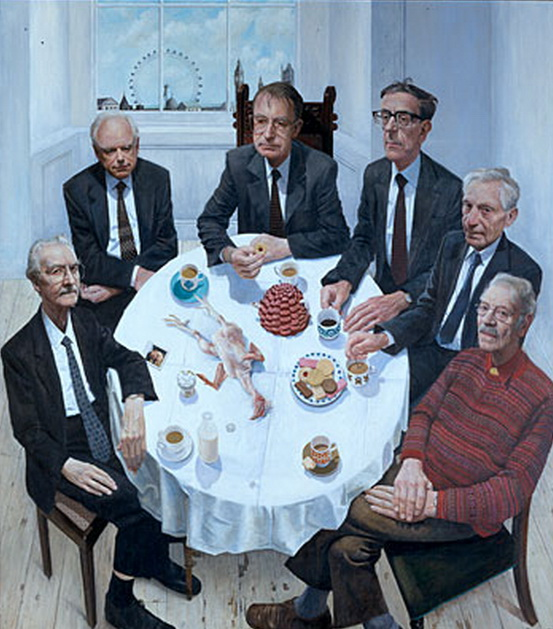
\includegraphics[height=\textheight]{stuartpearson}
\clearpage

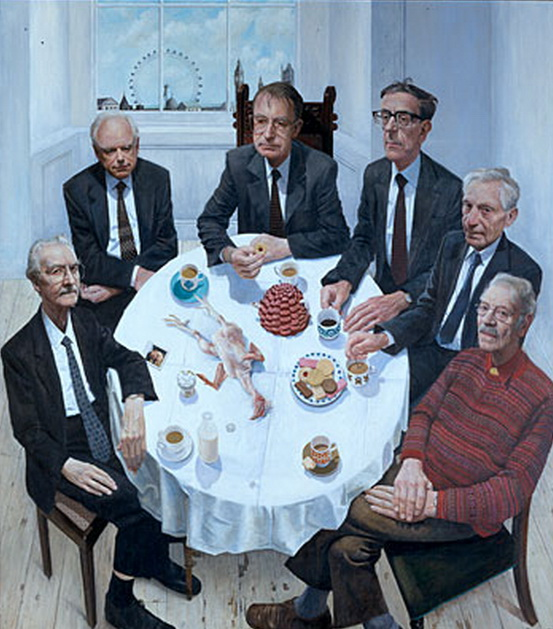
\includegraphics[height=\textheight]{stuartpearson}


%\restoregeometry

\newpage \newpage

\def\tol{3mm}
%\def\printlayout{%
%\begin{tikzpicture}[scale=0.6,font={\footnotesize\sffamily},line width=.6pt]
%\coordinate (pageX1) at (0,\paperheight);
%\coordinate (text1) at (1in+\innermargin,\paperheight-1in-\topmargin-\headsep-\headheight);
%% origin
%\draw [fill=black] (0,0) circle (3.5pt); 
%% draw paper
%\draw (pageX1) rectangle ++(\paperwidth, -\paperheight);
%% draw one inch around
%\draw [color=gray] (1in, 0) -- ++(0, \paperheight);
%\draw [color=gray] (0, \paperheight-1in) -- ++ (\paperwidth,0);
%% draw textarea
%\draw [color=green] (text1) rectangle ++ (\textwidth ,-\textheight);
%% oddside margin
%%\draw [color=blue] (1in+\innermargin, \paperheight-1in-\headsep-\headheight) -- ++ (0,-\textheight);
%% marginpar
%\draw [color=blue] (1in+\innermargin+\textwidth+\marginparsep,\paperheight-1in-\topmargin-\headsep-\headheight ) rectangle ++(\marginparwidth,-\textheight);
%% header
%%   top margin
%\draw [color=black] (1in + \innermargin+\tol, \paperheight-1in-\topmargin) 
%               -- ++ (\textwidth,0);
%\draw [color=black] (1in + \innermargin, \paperheight-1in-\topmargin ) 
%               rectangle ++ (\textwidth,-\headheight);
%% footer
%\draw (1in+\innermargin,\paperheight-1in-\topmargin-\headheight-\headsep-\textheight-\footskip)
%         -- ++ (\textwidth,0);
%% legends and dimensions top x-axis
%\draw (0,\paperheight+\tol)
%        -- ++(0,.8) 
%       ++ (1in, -0.8)
%       -- ++(0,0.8) node[ left=2mm]{1inch}; 
% \draw (-0.4,\paperheight+3mm+4mm) -- ++ (\paperwidth-\marginparwidth+2*\marginparsep,0);% horizontal line
% % back
%\draw (0+1in,\paperheight+3mm)--++(0,8mm);
%\draw (0+1in+\oddsidemargin,\paperheight+3mm)--++(0,8mm)
%         node[ right]{oddsidemargin=\the\oddsidemargin};
%% margin sep ticks
%\draw (1in+\oddsidemargin+\textwidth,\paperheight+\tol) -- ++ (0,20mm)++(0,-0.23) node [ left]{marginparsep=\the\marginparsep};
%\draw (1in+\oddsidemargin+\textwidth+\marginparsep,\paperheight+\tol) -- ++ (0,20mm);
%% marginpar ticks
%\draw (1in+\oddsidemargin+\textwidth+\marginparsep+\marginparwidth,\paperheight+\tol) 
%     -- ++ (0,20mm)
%         ++ (-\marginparwidth-\marginparsep-\tol,-0.5cm)
%     --  ++ (\marginparsep+\marginparwidth+4*\tol,0) ++(18mm,3mm) node {marginparwidth=\the\marginparwidth};
% % ticks on y-axis right
%\draw (\paperwidth+\tol,\paperheight)
%        -- ++ (0.8,0) 
%        ++ (-0.8,-1in-\topmargin)
%        --++(0.8,0)  node  [below right]{headheight = \the\headheight}
%        ++ (-0.8,-\headheight) 
%     -- ++(0.8,0)
%        ++ (-0.8,-\headsep) -- ++ (0.8,0) node [above right]{headsep = \the\headsep}
%
%        ++ (-0.8,-\textheight) -- ++ (0.8,0) node[right] at ++(0,0.5\textheight){textheight=\the\textheight}
%        ++ (-0.8, -\footskip) -- ++ (0.8,0)node [above right]{footskip = \the\footskip}
%        (\paperwidth+7mm,\footskip-3mm)-- ++ (0,\paperheight+0.4);  
%% bottom dimensions
%\draw (-3mm,- 10mm) -- ++(1in+1cm,0) node[above] at ++(-0.5in-0.5cm,0){1 inch}(1in,-8.3mm)--++(0,-0.8cm);  
%\draw (0,-8mm)-- 
%       ++(0, -2.5cm)++(\paperwidth,2.5cm)--++(0,-2.5cm); 
%\draw (-3mm,-2.5cm)--++(\paperwidth+6mm,0);
%\node[above] at (-3mm+0.5\paperwidth, -2.5cm) {paper width = \the\paperwidth};  
%%% left tick marks
%\draw (-3mm,0)-- (-1.3cm,0)++(0,\paperheight)--++(1cm,0);
%\draw [color=blue] (-7.8mm, -0.4) -- (-7.8mm,\paperheight + 0.4cm);
%% legend
%\node[rotate=90] at (-12.8mm, 0.5\paperheight){paper height = \the\paperheight};
%\end{tikzpicture}
%
%\clearpage
%\printgeometryvalues}

\printlayout\clearpage

\printlayout

\printgeometryvalues
\footnote{This is the first footnote}\footnote{This is the first footnote}\footnote{This is the first footnote}\footnote{This is the first footnote}\footnote{This is the first footnote}

%\begin{verbatim}
%\begin{teX}
%\if@compatibility
%  \setlength\topmargin{.75in}
%\else
%  \setlength\topmargin{\paperheight}
%  \addtolength\topmargin{-2in}
%  \addtolength\topmargin{-\headheight}
%  \addtolength\topmargin{-\headsep}
%  \addtolength\topmargin{-\textheight}
%  \addtolength\topmargin{-\footskip}     % this might be wrong! (previously set at 0.35in)
%  \addtolength\topmargin{-.5\topmargin}
%  \@settopoint\topmargin
%\fi
%\end{teX}
%
%\end{verbatim}
% \section{Paragraphs}
\bigskip

\parindent1em
\begin{tikzpicture}
\parindent1em
\def\parindent@cx{\the\parindent+3em}

\draw [->] (0-\parindent@cx,0)  circle (3.5pt) -- ++(\textwidth,0) -- ++ (0,0.15\textheight)
              -- ++ (-\textwidth+\parindent@cx,0) -- ++ (0,-\baselineskip)-- ++(-\parindent@cx,0)--++(0,-0.15\textheight+\baselineskip);

\def\parindent@cx{0cm}
\draw [color=blue!75,->] (0+1cm,-3.2cm)  circle (3.5pt) -- ++(\textwidth,0) -- ++ (0,0.15\textheight)
              -- ++ (-\textwidth+\parindent@cx,0) -- ++ (0,-\baselineskip)-- ++(-\parindent,0)--++(0,-0.15\textheight+\baselineskip);
\end{tikzpicture}

\end{document} 